\documentclass[12pt]{article}
\usepackage{graphics}
\usepackage[top=1in,bottom=1in,left=1in,right=1in]{geometry}
\usepackage{alltt}
\usepackage{array}	
\usepackage{graphicx}
\usepackage{tabularx}
\usepackage{verbatim}
\usepackage{setspace}
\usepackage{listings}

\usepackage{amssymb,amsmath, amsthm}
\usepackage{zed-csp}
\usepackage[cc]{titlepic}

\title{COMP 335: Introduction to Theoretical Computer Science\\
\ \\
Assignment 4}
\author{Nathan Grenier}
\date{\today \\ Fall 2024}

\begin{document}
\begin{spacing}{1.5}
      \maketitle

      \newpage

      \begin{enumerate}

            \item[1.] [20 Points]

                  \begin{enumerate}
                        \item[(a)] (10 Points)



                              % \begin{figure}[h!]
                              %       \centering
                              %       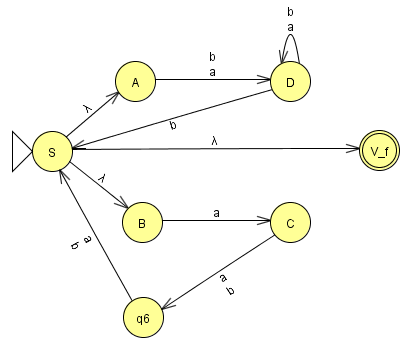
\includegraphics[width=0.65\textwidth]{img/q1/q1a(NFA).png}
                              % \end{figure}

                  \end{enumerate}

                  \newpage
            \item[2.] [25 Points]

                  \begin{enumerate}
                        \item[(a)] (5 Points)
                  \end{enumerate}

                  \newpage
            \item[3.] [20 Points]

                  \begin{enumerate}
                        \item[(a)] (10 Points)
                  \end{enumerate}

      \end{enumerate}

\end{spacing}

\end{document}